\newcommand{\posterAcknowledgments}[1]{

\setlength{\frameWidth}{#1}
\setlength{\unitlength}{0.02\frameWidth}
\psset{unit=\unitlength}

\rput[lt](1,31){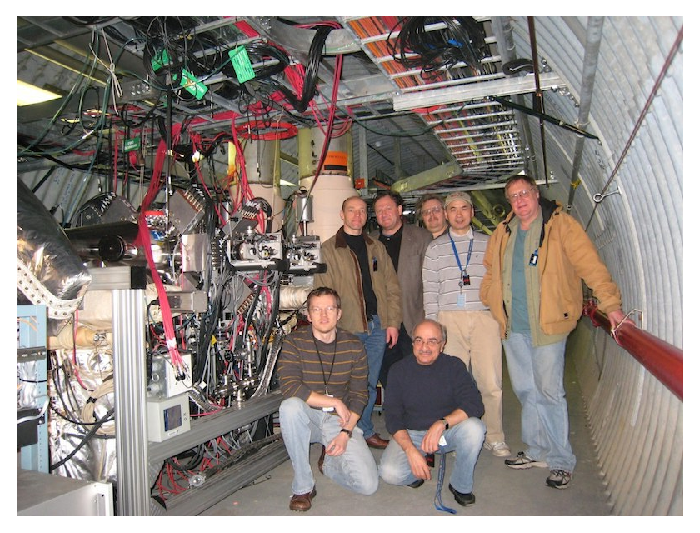
\includegraphics[width=25\unitlength]{graphics/Polarimetry_group}}

\rput[lt](29,27.5) {%
\begin{minipage}{21\unitlength}
\raggedright
\begin{list}{\labelitemi}{\setlength{\itemsep}{-3mm}
                          \setlength{\topsep}{0mm}
                          \setlength{\leftmargin}{0mm}
                          \setlength{\rightmargin}{0mm} }

\item I would like to thank the \textbf{Instrumentation Division} and
\textbf{Collider Accelerator Department} at BNL for their work on the silicon
detectors, electronics, and the RHIC polarized proton beam

\end{list}
\end{minipage}
}

\rput[lt](2,11) {%
\begin{minipage}{47\unitlength}
\raggedright
\begin{list}{\labelitemi}{\setlength{\itemsep}{0mm}
                          \setlength{\topsep}{0mm}
                          \setlength{\leftmargin}{0mm}
                          \setlength{\rightmargin}{0mm} }

\item I am thankful for discussions with the members of the \textbf{RHIC Spin
Collaboration}, in particular\\[\unitlength]
\small
\textbf{E.~Aschenauer, I.~Alekseev, M.~Bai, S.~Bazilevsky
W.~Fischer, H.~Huang, Y.~Makdisi, A.~Poblaguev, T.~Roser, B.~Schmidke,
D.~Svirida, and A.~Zelenski}
\normalsize

%\item {\small This work is performed under the auspices of U.S. DOE Contract No DE-AC02-98CH10886}

\end{list}
\end{minipage}
}

\rput(25,1){ \underline{\url{http://www.phy.bnl.gov/cnipol/}} }


%\rput{0}{\psgrid[gridlabels=0.7,subgriddiv=0, griddots=3](1,-1)(0,0)(\myPsPictureWidthLocal,\myPsPictureHeightLocal)}

}

\setlength{\unitlength}{10mm}
\psset{unit=\unitlength}
